\documentclass{standalone}
\usepackage{tikz}
\usetikzlibrary{shapes.geometric, arrows, positioning}
\usetikzlibrary{decorations.pathreplacing}
\usetikzlibrary{calc}

\tikzset{
    block/.style = {rectangle, minimum width=2.5cm, minimum height=1cm, text centered, draw=black,thick, fill=blue!60},
    endpoint/.style = {rectangle, text width=2.0cm, minimum width=1.5cm, minimum height=1cm, text centered, draw=black, fill=green!30},
    switch/.style = {regular polygon, regular polygon sides=6, minimum size=2.5cm, text centered, draw=black, fill=blue!50},
    arrow/.style = {thick,->,>=stealth},
    dashed_arrow/.style = {thick,dashed,->,>=stealth},
    brace/.style = {decorate,decoration={brace,amplitude=10pt,mirror,raise=1.5cm}},
    empty-block/.style = {rectangle, minimum width=1.5cm, minimum height=0.5cm, text centered, draw=black,thick, fill=green!50},
    label/.style = {midway, right=2cm,text width=3cm }
}

\begin{document}

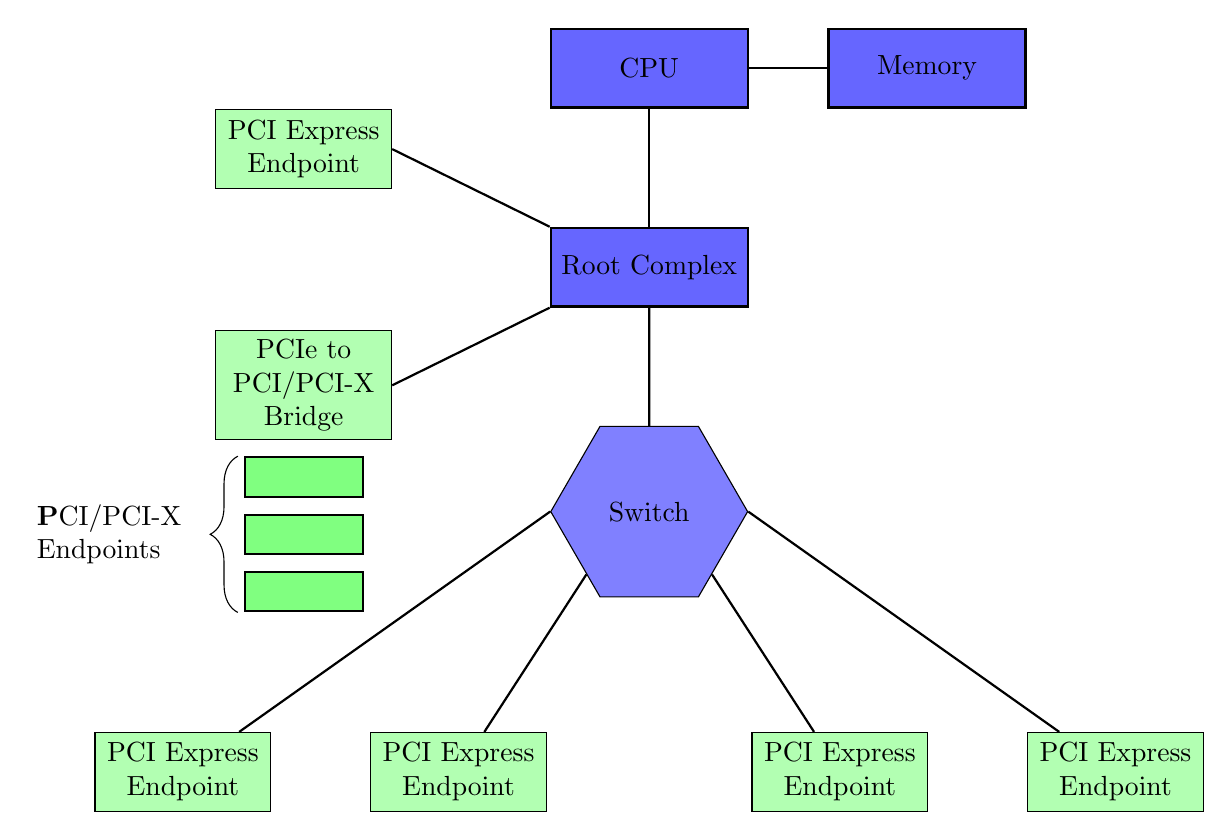
\begin{tikzpicture}[node distance=1.5cm and 1cm]

% below right=\verdist and \hordist of conc
% Nodes
\node (cpu) [block] {CPU};
\node (memory) [block, right=of cpu] {Memory};
\node (root) [block, below=of cpu] {Root Complex};
\node (switch) [switch, below=of root] {Switch};

\node (endpoint1) [endpoint, left=2cm of root, yshift=1.5cm] {PCI Express Endpoint};
\node (bridge) [endpoint, left=2cm of root, yshift=-1.5cm] {PCIe to PCI/PCI-X Bridge};

\node (endpoint2) [endpoint, below right=2cm and 0.5cm of switch] {PCI Express Endpoint};
\node (endpoint3) [endpoint, below right=2cm and 4cm of switch] {PCI Express Endpoint};
\node (endpoint4) [endpoint, below left=2cm and 0.5cm of switch] {PCI Express Endpoint};
\node (endpoint5) [endpoint, below left=2cm and 4cm of switch] {PCI Express Endpoint};

% \node (pcix_endpoints) [endpoint, left=of bridge, yshift=-1.5cm] {PCI/PCI-X Endpoints};
\node (endpoint6) [empty-block, below=0.2cm of bridge] {};
\node (endpoint7) [empty-block, below=0.2cm of endpoint6] {};
\node (endpoint8) [empty-block, below=0.2cm of endpoint7] {};

% Brace
\draw [brace] ($(endpoint6.north east) + (-0.1, 0)$) -- ($(endpoint8.south east) + (-0.1,0)$) node [label] {};

\node [left=0.5cm of endpoint7, text width=2cm] { {\textbf PCI/PCI-X Endpoints}};

% Connections
\draw [thick] (cpu) -- (root);
\draw [thick] (cpu) -- (memory);
\draw [thick] (root) -- (switch);
\draw [thick] (root.north west) -- (endpoint1.east);
\draw [thick] (root.south west) -- (bridge.east);
\draw [thick] (switch.south east) -- (endpoint2);
\draw [thick] (switch.east) -- (endpoint3);
\draw [thick] (switch.south west) -- (endpoint4);
\draw [thick] (switch.west) -- (endpoint5);

% \draw [dashed] (bridge) -- ++(-1.5,0) -- ++(0,-1.5) -- ++(3,0) -- ++(0,1.5);
% \draw [dashed_arrow] (bridge) -- (pcix_endpoints);

\end{tikzpicture}

\end{document}
